%
% $RCSfile: broker.tex,v $
%
% Copyright (c) 2004. Christian Heller. All rights reserved.
%
% No copying, altering, distribution or any other actions concerning this
% document, except after explicit permission by the author!
% At some later point in time, this document is planned to be put under
% the GNU FDL license. For now, _everything_ is _restricted_ by the author.
%
% http://www.cybop.net
% - Cybernetics Oriented Programming -
%
% http://www.resmedicinae.org
% - Information in Medicine -
%
% @author Christian Heller <christian.heller@tuxtax.de>
%

\paragraph{Broker}
\label{broker_heading}

The \emph{Broker} pattern \cite{buschmann} may support the creation of an IT
infrastructure for distributed applications. It connects decoupled components
which interact through remote service invocations (figure \ref{broker_figure}).

\begin{figure}[ht]
    \begin{center}
        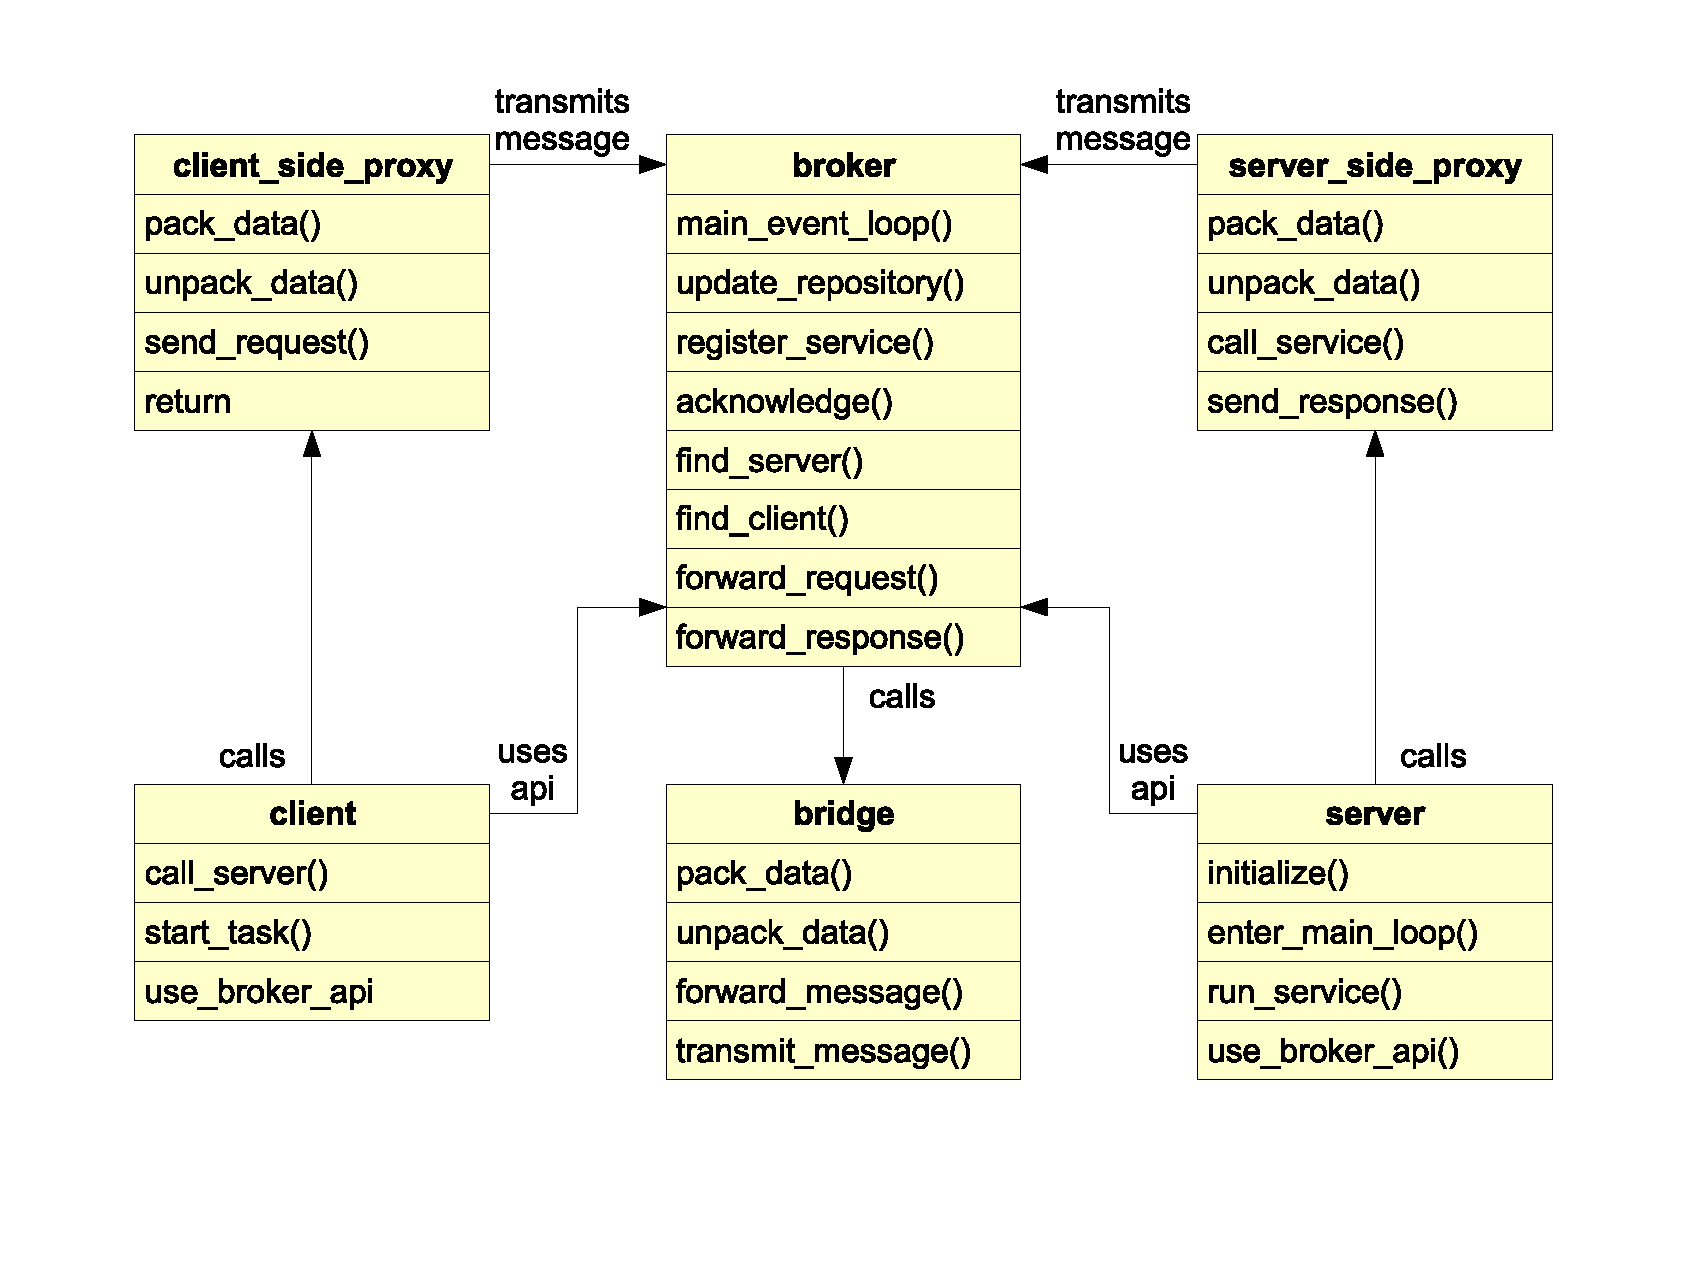
\includegraphics[scale=0.3]{vector/broker.eps}
        \caption{Broker Pattern}
        \label{broker_figure}
    \end{center}
\end{figure}

The broker is responsible for coordinating all communication, for forwarding
requests as well as for transmitting results and exceptions.
